\section{Stars and Galaxies}
\subsection{The Life Cycle of Stars}
Stars are massive celestial objects primarily composed of hydrogen and helium. They generate energy through \textbf{nuclear fusion}. The evolution of a star depends largely on its \textit{initial mass}.

\textcite{carroll2007} describe stellar structure and evolution in detail.

\subsection{Types of Galaxies}
Galaxies can be classified into several major categories:
\begin{itemize}
    \item Spiral galaxies
    \item Elliptical galaxies
    \item Irregular galaxies
\end{itemize}

\begin{figure}[htbp]
    \centering
    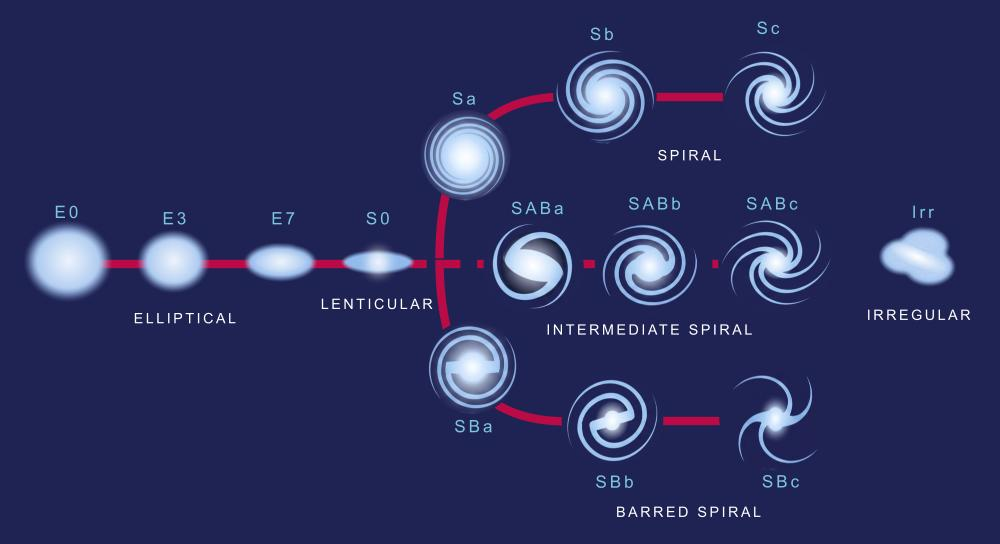
\includegraphics[width=0.8\textwidth]{figures/images/galaxy-types.jpg}
    \caption{Major galaxy morphologies: spiral, elliptical, and irregular.}
    \label{fig:galaxy-types}
\end{figure}